\chapter{Transport Protocols}
\label{cha:transport-protocols}

\section{TCP}
\label{sec:tcp}

\subsection{Overview}
\label{sec:tcp_overview}

The \nedtype{Tcp} simple module is the primary implementation 
of the TCP protocol in the INET framework.

INET contains two other implementation of the TCP protocol:
\nedtype{TCP\_lwIP} and \nedtype{TCP\_NSC}, which are based
on external codebases.

All TCP modules implements the \nedtype{ITcp} interface and
communicate with the application and the IP layer through the
same interface, so they can be interchanged and can also be 
mixed in the same network.

\subsection{Protocol Overview}
\label{sec:tcp_prot}

TCP protocol is the most widely used protocol of the Internet. It provides
reliable, ordered delivery of stream of bytes from one application on one computer
to another application on another computer. It is used by such applications as
World Wide Web, email, file transfer amongst others.

The baseline TCP protocol is described in RFC793, but other tens of RFCs
contains modifications and extensions to the TCP. These proposals
enhance the efficiency and safety of the TCP protocol and they are widely
implemented in the real TCP modules. As a result, TCP is a complex protocol
and sometimes it is hard to see how the different requirements interacts
with each other.

The TCP modules of the INET framework implements the following RFCs:

\begin{tabular}{ll}
RFC 793 & Transmission Control Protocol \\
RFC 896 & Congestion Control in IP/TCP Internetworks \\
RFC 1122 & Requirements for Internet Hosts -- Communication Layers \\
RFC 1323 & TCP Extensions for High Performance \\
RFC 2018 & TCP Selective Acknowledgment Options \\
RFC 2581 & TCP Congestion Control \\
RFC 2883 & An Extension to the Selective Acknowledgement (SACK) Option for TCP \\
RFC 3042 & Enhancing TCP's Loss Recovery Using Limited Transmit \\
RFC 3390 & Increasing TCP's Initial Window \\
RFC 3517 & A Conservative Selective Acknowledgment (SACK)-based Loss Recovery \newline
                 Algorithm for TCP \\
RFC 3782 & The NewReno Modification to TCP's Fast Recovery Algorithm \\
\end{tabular}

In this section we describe the features of the TCP protocol specified by these RFCs,
the following sections deal with the implementation of the TCP in the INET framework.

\subsubsection{TCP segments}

The TCP module transmits a stream of the data over the unreliable, datagram service
that the IP layer provides. When the application writes a chunk of data into the socket,
the TCP module breaks it down to packets and hands it over the IP. On the receiver side,
it collects the recieved packets, order them, and acknowledges the reception. The packets
that are not acknowledged in time are retransmitted by the sender.

The TCP procotol can address each byte of the data stream by \emph{sequence numbers}.
The sequence number is a 32-bit unsigned integer, if the end of its range is reached,
it is wrapped around.

The layout of the TCP segments is described in RFC793:

\begin{center}
\begin{bytefield}{32}
\bitheader{0,3,4,7,8,15,16,31} \\
\bitbox{16}{Source Port} &
\bitbox{16}{Destination Port} \\
\bitbox{32}{Sequence Number} \\
\bitbox{32}{Acknowledgment Number} \\
\bitbox{4}{\small Data Offset} &
\bitbox{6}{Reserved} &
\bitbox{6}{Flags} &
\bitbox{16}{Window} \\
\bitbox{16}{Checksum} &
\bitbox{16}{Urgent Pointer} \\
\bitbox{24}{Options} &
\bitbox{8}{Padding} \\
\wordbox{3}{Data}
\end{bytefield}
\end{center}

Here
\begin{itemize}
  \item the Source and Destination Ports, together with the Source and Destination
  addresses of the IP header identifies the communication endpoints.
  \item the Sequence Number identifier of the first data byte transmitted in the sequence,
  Sequence Number + 1 identifies the second byte, so on. If the SYN flag is set it consumes
  one sequence number before the data bytes.
  \item the Acknowlegment Number refers to the next byte (if the ACK flag is set) expected
  by the receiver using its sequence number
  \item the Data Offset is the length of the TCP header in 32-bit words (needed because the
  Options field has variable length)
  \item the Reserved bits are unused
  \item the Flags field composed of 6 bits:
  \begin{itemize}
    \item URG: Urgent Pointer field is significant
    \item ACK: Acknowledgment field is significant
    \item PSH: Push Function
    \item RST: Reset the connection
    \item SYN: Synchronize sequence number
    \item FIN: No more data from sender
  \end{itemize}
  \item the Window is the number of bytes the receiver TCP can accept (because of its
  limited buffer)
  \item the Checksum is the 1-complement sum of the 16-bit words of the IP/TCP header and
  data bytes
  \item the Urgent Pointer is the offset of the urgent data (if URG flag is set)
  \item the Options field is variable length, it can occupy 0-40 bytes in the header and is
  always padded to a multiple of 4 bytes.
\end{itemize}

\subsubsection{TCP connections}

When two applications are communicating via TCP, one of the applications is the client,
the other is the server. The server usually starts a socket with a well known local port
and waits until a request comes from clients. The client applications are issue connection
requests to the port and address of the service they want to use.

After the connection is established both the client and the server can send and receive data.
When no more data is to be sent, the application closes the socket. The application can still
receive data from the other direction. The connection is closed when both communication partner
closed its socket.

...

When opening the connection an initial sequence number is choosen and communicated to the
other TCP in the SYN segment. This sequence number can not be a constant value (e.g. 0),
because then data segments from a previous incarnation of the connection (i.e. a connection
with same addresses and ports) could be erronously accepted in this connection. Therefore
most TCP implementation choose the initial sequence number according to the system clock.


\begin{figure}
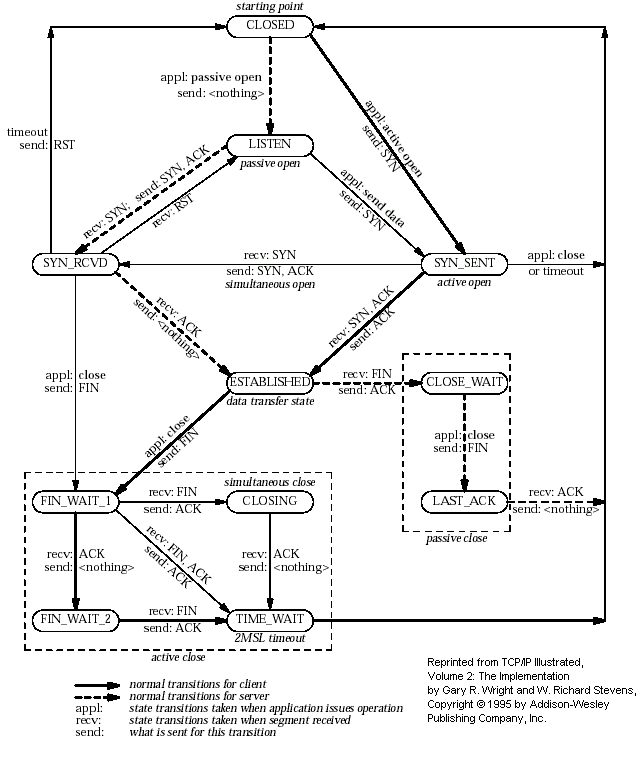
\includegraphics[width=\textwidth]{figures/tcpstate}
\caption{TCP state diagram}
\label{fig:tcp_states}
\end{figure}

\subsubsection{Flow control}
\label{subsec:flow_control}

The TCP module of the receiver buffers the data of incoming segments.
This buffer has a limited capacity, so it is desirable to notify the sender
about how much data the client can accept. The sender stops the transmission
if this space exhausted.

In TCP every ACK segment holds a Window field; this is the available space
in the receiver buffer. When the sender reads the Window, it can send at most
Window unacknowledged bytes.

\subsubsection*{Window Scale option}

% RFC1323
The TCP segment contains a 16-bit field for the Window, thus allowing at most
65535 byte windows. If the network bandwidth and latency is large, it is surely
too small. The sender should be able to send bandwitdh*latency bytes without
receiving ACKs.

For this purpose the Window Scale (WS) option had been introduced in RFC1323.
This option specifies a scale factor used to interpret the value of the Window field.
The format is the option is:

\begin{center}
\begin{bytefield}{24}
\bitbox{8}{Kind=3} &
\bitbox{8}{Length=3} &
\bitbox{8}{shift.cnt}
\end{bytefield}
\end{center}

If the TCP want to enable window sizes greater than 65535, it should send
a WS option in the SYN segment or SYN/ACK segment (if received a SYN with WS
option). Both sides must send the option in the SYN segment to enable window scaling,
but the scale in one direction might differ from the scale in the other direction.
The $shift.cnt$ field is the 2-base logarithm of the window scale of the sender.
Valid values of $shift.cnt$ are in the $[0,14]$ range.

\subsubsection*{Persistence timer}

When the reciever buffer is full, it sends a 0 length window in the ACK segment
to stop the sender. Later if the application reads the data,
it will repeat the last ACK with an updated window to resume data sending.
If this ACK segment is lost, then the sender is not notified, so a deadlock
happens.

To avoid this situation the sender starts a Persistence Timer when it received
a 0 size window. If the timer expires before the window is increased it send
a probe segment with 1 byte of data. It will receive the current window of the
receiver in the response to this segment.

\subsubsection*{Keepalive timer}

TCP keepalive timer is used to detect dead connections.

\subsubsection{Transmission policies}
\label{subsec:trans_policies}

\subsubsection*{Retransmissions}

% source: RFC1222 4.3.2.1 and Tannenbaum 6.5.10

When the sender TCP sends a TCP segment it starts a
retransmission timer.
If the ACK arrives before the timer expires it is stopped,
otherwise it triggers a retransmission of the segment.

If the retransmission timeout (RTO) is too high, then lost segments
causes high delays, if it is too low, then the receiver gets
too many useless duplicated segments. For optimal behaviour, the
timeout must be dynamically determined.

Jacobson suggested to measure the RTT mean and deviation
and apply the timeout:

$$ RTO = RTT + 4 * D $$

Here RTT and D are the measured smoothed roundtrip time and its
smoothed mean deviation. They are initialized to 0 and updated each time an
ACK segment received according to the following formulas:

$$ RTT = \alpha*RTT + (1-\alpha) * M $$

$$ D = \alpha*D + (1-\alpha)*|RTT-M| $$

where $M$ is the time between the segments send and the acknowledgment
arrival. Here the $\alpha$ smoothing factor is typically $7/8$.

One problem may occur when computing the round trip: if the
retransmission timer timed out and the segment is sent again,
then it is unclear that the received ACK is a response to the
first transmission or to the second one. To avoid confusing the
RTT calculation, the segments that have been retransmitted
do not update the RTT. This is known as Karn's modification.
He also suggested to double the $RTO$ on each failure until the
segments gets through (``exponential backoff'').

\subsubsection*{Delayed ACK algorithm}

% RFC1122 4.2.3.2

A host that is receiving a stream of TCP data segments can
increase efficiency in both the Internet and the hosts by
sending fewer than one ACK (acknowledgment) segment per data
segment received; this is known as a "delayed ACK" [TCP:5].

Delay is max. 500ms.

A delayed ACK gives the application an opportunity to
update the window and perhaps to send an immediate
response.  In particular, in the case of character-mode
remote login, a delayed ACK can reduce the number of
segments sent by the server by a factor of 3 (ACK,
window update, and echo character all combined in one
segment).

In addition, on some large multi-user hosts, a delayed
ACK can substantially reduce protocol processing
overhead by reducing the total number of packets to be
processed [TCP:5].  However, excessive delays on ACK's
can disturb the round-trip timing and packet "clocking"
algorithms [TCP:7].

% RFC2581 3.2

a TCP receiver SHOULD send an immediate ACK
when the incoming segment fills in all or part of a gap in the
sequence space.

\subsubsection*{Nagle's algorithm}

RFC896 describes the ``small packet problem": when the application
sends single-byte messages to the TCP, and it transmitted immediatly
in a 41 byte TCP/IP packet (20 bytes IP header, 20 bytes TCP header,
1 byte payload), the result is a 4000\% overhead that can cause
congestion in the network.

The solution to this problem is to delay the transmission until
enough data received from the application and send all collected
data in one packet. Nagle proposed that
when a TCP connection has outstanding data that has not
yet been acknowledged, small segments should not be sent
until the outstanding data is acknowledged.

\subsubsection*{Silly window avoidance}

The Silly Window Syndrome (SWS) is described in RFC813. It occurs when
a TCP receiver advertises a small window and the TCP sender immediately
sends data to fill the window. Let's take the example when the sender
process writes a file into the TCP stream in big chunks, while the
receiver process reads the bytes one by one. The first few bytes
are transmitted as whole segments until the receiver buffer
becomes full. Then the application reads one
byte, and a window size 1 is offered to the sender. The sender sends
a segment with 1 byte payload immediately, the receiver buffer becomes
full, and after reading 1 byte, the offered window is 1 byte again.
Thus almost the whole file is transmitted in very small segments.

In order to avoid SWS, both sender and receiver must try to avoid this
situation. The receiver must not advertise small windows and the sender
must not send small segments when only a small window is advertised.

In RFC813 it is offered that
\begin{enumerate}
  \item the receiver should not advertise windows that is smaller than the maximum
        segment size of the connection
  \item the sender should wait until the window is large enough for a maximum sized
        segment.
\end{enumerate}

\subsubsection*{Timestamp option}

Efficient retransmissions depends on precious RTT measurements.
Packet losses can reduce the precision of these measurements radically.
When a segment lost, the ACKs received in that window can not be used;
thus reducing the sample rate to one RTT data per window. This is
unacceptable if the window is large.

The proposed solution to the problem is to use a separate timestamp
field to connect the request and the response on the sender side.
The timestamp is transmitted as a TCP option. The option contains two
32-bit timestamps:

\begin{center}
\begin{bytefield}{80}
\bitbox{8}{Kind=5} &
\bitbox{8}{Length=10} &
\bitbox{32}{TS Value} &
\bitbox{32}{TS Echo Reply} &
\end{bytefield}
\end{center}

Here the TS Value (TSVal) field is the current value of the timestamp
clock of the TCP sending the option, TS Echo Reply (TSecr) field is
0 or echoes the timestamp value of that was sent by the remote TCP.
The TSscr field is valid only in ACK segments that acknowledges new
data. Both parties should send the TS option in their SYN segment
in order to allow the TS option in data segments.

The timestamp option can also be used for PAWS (protection against wrapped
sequence numbers).


\subsubsection{Congestion control}

Flow control allows the sender to slow down the transmission when the
receiver can not accept them because of memory limitations. However
there are other situations when a slow down is desirable. If the sender
transmits a lot of data into the network it can overload the processing
capacities of the network nodes, so packets are lost in the network
layer.

For this purpose another window is maintained at the sender side, the
congestion window (CWND). The congestion window is a sender-side limit
on the amount of data the sender can transmit into the network before
receiving ACK. More precisely, the sender can send at most max(CWND, WND)
bytes above SND.UNA, therefore $ SND.NXT < SND.UNA + max(CWND, WND) $ is
guaranteed.

The size of the congestion window is dinamically determined by monitoring
the state of the network.

% RFC2581
%
% Definitions:
% SMSS: sender maximum segment size
% RMSS: receiver maximum segment size (default 536)
% rwnd: most recently advertised receiver window
% IW: initial sender's congestion window
% LW: loss window, size of congestion window after a TCP sender detects loss
% RW: restart window, size of congestion window after a TCP restarts transmission after an idle period
% fligth size: amount of data has been sent but not yet acknowledged
% cwnd: congestion window, sender-size limit on the amount of data the sender
%       can transmit into the network before receiving an ACK
% rwnd: receiver advertised window, receiver-side limit on the amount of outstanding data
% sstresh: whether slow start or congestion avoidance used
%
% IW <= 2*MSS


\subsubsection*{Slow Start and Congestion Avoidance}

There are two algorithm that updates the congestion window, ``Slow Start''
and ``Congestion Avoidance''. They are specified in RFC2581.

\begin{pseudocode}
$cwnd \gets 2*SMSS$
$ssthresh \gets $ upper bound of the window (e.g. $65536$)
whenever ACK received
  if $cwnd < ssthresh$
    $cwnd \gets cwnd + SMSS$
  otherwise
    $cwnd \gets cwnd + SMSS*SMSS/cwnd$
whenever packet loss detected
  $cwnd \gets SMSS$
  $ssthresh \gets max(FlightSize/2, 2*SMSS)$
\end{pseudocode}

Slow Start means that when the connection opened the sender initially
sends the data with a low rate. This means that the initial
window (IW) is at most 2 MSS, but no more than 2 segments. If there was no packet loss,
then the congestion window is increased rapidly, it is doubled in each flight.
When a packet loss is detected, the congestion window is reset to 1 MSS (loss window, LW)
and the ``Slow Start'' is applied again.

\begin{note}
RFC3390 increased the IW to roughly 4K bytes: $min(4*MSS, max(2*MSS, 4380))$.
\end{note}

When the congestion window reaches a certain limit (slow start threshold),
the ``Congestion Avoidance'' algorithm is applied. During ``Congestion Avoidance''
the window is incremented by 1 MSS per round-trip-time (RTT). This is usually
implemented by updating the window according to the $ cwnd += SMSS*SMSS/cwnd $
formula on every non-duplicate ACK.

The Slow Start Threshold is updated when a packet loss is detected.
It is set to $max(FlightSize/2, 2*SMSS)$.

How the sender estimates the flight size? The data sent, but not yet acknowledged.

How the sender detect packet loss? Retransmission timer expired.


\subsubsection*{Fast Retransmit and Fast Recovery}

RFC2581 specifies two additional methods to increase the efficiency
of congestion control: ``Fast Retransmit'' and ``Fast Recovery''.

``Fast Retransmit'' requires that the receiver signal the event,
when an out-of-order segment arrives. It is achieved by sending
an immediate duplicate ACK. The receiver also sends an immediate
ACK when the incoming segment fills in a gap or part of a gap.

When the sender receives the duplicated ACK it knows that some
segment after that sequence number is received out-of-order or
that the network duplicated the ACK. If 3 duplicated ACK received
then it is more likely that a segment was dropped or delayed.
In this case the sender starts to retransmit the segments
immediately.

``Fast Recovery'' means that ``Slow Start'' is not applied
when the loss is detected as 3 duplicate ACKs. The arrival
of the duplicate ACKs indicates that the network is not fully
congested, segments after the lost segment arrived, as well
the ACKs.

% Details?
%
%    1.  When the third duplicate ACK is received, set ssthresh to no more
%        than the value given in equation 3.
%
%    2.  Retransmit the lost segment and set cwnd to ssthresh plus 3*SMSS.
%        This artificially "inflates" the congestion window by the number
%        of segments (three) that have left the network and which the
%        receiver has buffered.
%
%    3.  For each additional duplicate ACK received, increment cwnd by
%        SMSS.  This artificially inflates the congestion window in order
%        to reflect the additional segment that has left the network.
%
%    4.  Transmit a segment, if allowed by the new value of cwnd and the
%        receiver's advertised window.
%
%    5.  When the next ACK arrives that acknowledges new data, set cwnd to
%        ssthresh (the value set in step 1).  This is termed "deflating"
%        the window.
%
%        This ACK should be the acknowledgment elicited by the
%        retransmission from step 1, one RTT after the retransmission
%        (though it may arrive sooner in the presence of significant out-
%        of-order delivery of data segments at the receiver).
%        Additionally, this ACK should acknowledge all the intermediate
%        segments sent between the lost segment and the receipt of the
%        third duplicate ACK, if none of these were lost.

\subsubsection*{Loss Recovery Using Limited Transmit}

If there is not enough data to be send after a lost segment,
then the Fast Retransmit algorithm is not activated, but the
costly retranmission timeout used.

RFC3042 suggests that the sender TCP should send a new data segment
in response to each of the first two duplicate acknowledgement. Transmitting
these segments increases the probability that TCP can recover from a single
lost segment using the fast retransmit algorithm, rather than using a costly
retransmission timeout.

\subsubsection*{Selective Acknowledgments}

% RFC2018

With selective
acknowledgments (SACK), the data receiver can inform the sender about all
segments that have arrived successfully, so the sender need
retransmit only the segments that have actually been lost.

With the help of this information the sender can detect
\begin{itemize}
  \item replication by the network
  \item false retransmit due to reordering
  \item retransmit timeout due to ACK loss
  \item early retransmit timeout
\end{itemize}


In the congestion control algorithms described so far
the sender has only rudimentary information about which
segments arrived at the receiver. On the other hand
the algorithms are implemented completely on the sender side,
they only require that the client sends immediate ACKs on
duplicate segments. Therefore they can work in a heterogenous
environment, e.g. a client with Tahoe TCP can communicate with
a NewReno server. On the other hand SACK must be supported by
both endpoint of the connection to be used.

If a TCP supports SACK it includes the \emph{SACK-Permitted} option
in the SYN/SYN-ACK segment when initiating the connection.
The SACK extension enabled for the connection if the \emph{SACK-Permitted}
option was sent and received by both ends. The option occupies
2 octets in the TCP header:

\begin{center}
\begin{bytefield}{16}
\bitbox{8}{Kind=4} &
\bitbox{8}{Length=2}
\end{bytefield}
\end{center}

If the SACK is enabled then the data receiver adds SACK option
to the ACK segments. The SACK option informs the sender about
non-contiguous blocks of data that have been received and queued.
The meaning of the \emph{Acknowledgement Number} is unchanged,
it is still the cumulative sequence number. Octets received
before the \emph{Acknowledgement Number} are kept by the receiver,
and can be deleted from the sender's buffer. However the receiver
is allowed to drop the segments that was only reported in the SACK
option.

The \emph{SACK} option contains the following fields:

\begin{center}
\begin{bytefield}{32}
\bitbox[]{16}{} &
\bitbox{8}{Kind=5} &
\bitbox{8}{Length} \\
\bitbox{32}{Left Edge of 1st Block} \\
\bitbox{32}{Right Edge of 1st Block} \\
\wordbox[]{1}{$\vdots$ \\[1ex]} \\
\bitbox{32}{Left Edge of nth Block} \\
\bitbox{32}{Right Edge of nth Block}
\end{bytefield}
\end{center}

Each block represents received bytes of data that are
contiguous and isolated with one exception: if a segment
received that was already ACKed (i.e. below $RCV.NXT$),
it is included as the first block of the \emph{SACK} option.
The purpose is to inform the sender about a spurious retransmission.

Each block in the option occupies 8 octets. The TCP header
allows 40 bytes for options, so at most 4 blocks can be
reported in the \emph{SACK} option (or 3 if TS option is also used).
The first block is used for reporting the most recently received
data, the following blocks repeats the most recently reported
SACK blocks. This way each segment is reported at least 3 times,
so the sender receives the information even if some ACK segment is
lost.


\textbf{SACK based loss recovery}

% RFC3517: loss recovery based on SACK

Now lets see how the sender can use the information in the
\emph{SACK} option. First notice that it can give a better
estimation of the amount of data outstanding in the network
(called $pipe$ in RFC3517).
If $highACK$ is the highest ACKed sequence number, and
$highData$ of the highest sequence number transmitted,
then the bytes between $highACK$ and $highData$ can be
in the network. However $ pipe \neq highData - highACK $
if there are lost and retransmitted segments:

$$ pipe = highData - highACK - lostBytes + retransmittedBytes $$

A segment is supposed to be lost if it was not received
but 3 segments recevied that comes after this segment in the sequence
number space.
This condition is detected by the sender by receiving
either 3 discontiguous SACKed blocks, or at least
$3*SMSS$ SACKed bytes above the sequence numbers of the
lost segment.

The transmission of data starts with a \emph{Slow Start} phase.
If the loss is detected by 3 duplicate ACK, the sender
goes into the recovery state: it sets
$cwnd$ and $ssthresh$ to $FlightSize / 2$.
It also remembers the $highData$ variable, because
the recovery state is left when this sequence number
is acknowledged.

In the recovery state it sends data
until there is space in the congestion window (i.e. $cwnd-pipe >= 1 SMSS$)
The data of the segment is choosen by the following rules (first rule that applies):

\begin{enumerate}
  \item send segments that is lost and not yet retransmitted
  \item send segments that is not yet transmitted
  \item send segments that is not yet retransmitted and possibly fills a gap
        (there is SACKed data above it)
\end{enumerate}

If there is no data to send, then the sender waits for the next ACK, updates
its variables based on the data of the received ACK, and then try to transmit
according to the above rules.

If an RTO occurs, the sender drops the collected SACK information and
initiates a Slow Start. This is to avoid a deadlock when the receiver
dropped a previously SACKed segment.

% highACK: highest ACKed sequence number
%
% highData: highest sequence number transmitted
%
% highRxt: highest sequence number which has been retransmitted
%
%
% Normal phase: before the first loss, until 3 duplicate ACK
%
% Loss recovery phase: until ACK for RecoveryPoint received
%
% On the transition to loss recovery phase
% \begin{enumerate}
%   \item RecoveryPoint=HighData
%   \item ssthresh=cwnd=FlightSize/2
%   \item compute \emph{pipe}
% \end{enumerate}
%
% In the loss recovery phase, for each incoming ACK:
%
% \begin{enumerate}
%   %\Alph
%   \item if cumulative ACK above RecoveryPoint, leave loss recovery phase
%   \item update SACK info and compute pipe
%   \item if $cwnd-pipe >= 1 SMSS$ send one or more segments (if there is data to send)
%   \item update HighRxt, HighData according to the sent bytes
%   \item increment $pipe$ by the amount of data sent
%   \item if $cwnd-pipe >= 1 SMSS$, continue sending
% \end{enumerate}
%
% Which bytes to be send are determined as follows:
%
% \begin{enumerate}
%   \item if there is a byte which is lost and not yet retransmitted, send that in 1 segment
%   \item otherwise if there is unsent data, send that in 1 segment
%   \item otherwise if there is not yet retransmitted data, and above that there is SACKed data, send that
%   \item otherwise there is no data to send
% \end{enumerate}


\subsection{The TCP module}
\label{sec:tcp_module}

The \nedtype{Tcp} simple module is the main implementation of the TCP protocol in the INET framework.
The \nedtype{Tcp} module as other transport protocols work above the network layer and below the application
layer, therefore it has gates to be connected with the IPv4 or IPv6 network (ipIn/ipOut or ipv6In/ipv6Out),
and with the applications (appIn[k], appOut[k]).
One \nedtype{Tcp} module can serve several application modules, and several
connections per application. The $k$th application connects to \nedtype{Tcp}'s
\ttt{appIn[k]} and \ttt{appOut[k]} ports.

The TCP module usually specified by its module interface
(\nedtype{ITcp}) in the NED definition of hosts, so it can be replaced with any implementation
that communicates through the same gates.

\subsubsection{Statistics}

The \nedtype{Tcp} module collects the following vectors:

\begin{tabular}{l p{10cm}}
  \ttt{send window} & $SND.WND$ \\
  \ttt{receive window} & $RCV.WND$, after SWS avoidance applied \\
  \ttt{advertised window} & $RCV.NXT + RCV.WND$ \\
  \ttt{sent seq} & \emph{Sequence Number} of the sent segment \\
  \ttt{sent ack} & \emph{Acknowledgement Number} of the sent segment \\
  \ttt{rcvd seq} & \emph{Sequence Number} of the received segment \\
  \ttt{rcvd ack} & \emph{Acknowledgement Number} of the received segment \\
  \ttt{unacked bytes} & number of sent and unacknowledged bytes ($max of SND.NXT - SND.UNA$) \\
  \ttt{rcvd dupAcks} & number of duplicate acknowledgements, reset to 0 when $SND.UNA$ advances \\
  \ttt{pipe} & the value of the SACK $pipe$ variable
               (estimated number of bytes outstanding in the network) \\
  \ttt{sent sacks} & number of SACK blocks sent \\
  \ttt{rcvd sacks} & number of SACK blocks received \\
  \ttt{rcvd oooseg} & number of received out-of-order segments \\
  \ttt{rcvd naseg} & number of received unacceptable segments (outside the receive window) \\
  \ttt{rcvd sackedBytes} & total amount of SACKed bytes in the buffer of the sender \\
  \ttt{tcpRcvQueueBytes} & number of bytes in the receiver's buffer \\
  \ttt{tcpRcvQueueDrops} & number of bytes dropped by the receiver (not enough buffer) \\
  \ttt{cwnd} & congestion window \\
  \ttt{ssthresh} & slow start threshold \\
  \ttt{measured RTT} & measured round trip time \\
  \ttt{smoothed RTT} & smoothed round trip time \\
  \ttt{RTTVAR} & measured smoothed variance of round trip time \\
  \ttt{RTO} & retransmission timeout \\
  \ttt{numRTOs} & number of retransmission timeouts occured \\
\end{tabular}

If the \fpar{recordStats} parameter is set to \fkeyword{false}, then none
of these output vectors are generated.

% \subsection{Animation effects}
%
% TCP module text: number of connections sorted by state
%
% log, log verbose

\subsection{TCP lwIP}
\label{sec:tcp_lwip}

lwIP is a light-weight implementation of the TCP/IP protocol suite
that was originally written by Adam Dunkels of the Swedish Institute of
Computer Science. The current development homepage is
\url{http://savannah.nongnu.org/projects/lwip/}.

The implementation targets embedded devices: it has
very limited resource usage (it works ``with tens of kilobytes of RAM and
around 40 kilobytes of ROM'') and does not require an underlying OS.

The \nedtype{TCP\_lwIP} simple module is based on the 1.3.2 version of
the lwIP sources.

Features:

\begin{compactitem}
\item delayed ACK
\item Nagle's algorithm
\item round trip time estimation
\item adaptive retransmission timeout
\item SWS avoidance
\item slow start threshold
\item fast retransmit
\item fast recovery
\item persist timer
\item keep-alive timer
\end{compactitem}

\subsubsection*{Limitations}

\begin{itemize}
  \item only MSS and TS TCP options are supported. The TS option is turned off
        by default, but can be enabled by defining LWIP\_TCP\_TIMESTAMPS to 1
        in \ffilename{lwipopts.h}.
  \item \fvar{fork} must be \fkeyword{true} in the passive open command
  \item The status request command (TCP\_C\_STATUS) only reports the
          local and remote addresses/ports of the connection and
          the MSS, SND.NXT, SND.WND, SND.WL1, SND.WL2, RCV.NXT, RCV.WND variables.
\end{itemize}

% lwIP license file missing from INET source
% FIXME TCP_lwIP uses only connId to identify the connection instead of (connId,appGateIndex)
% FIXME status command returns message kind TCP_C_STATUS instead of TCP_I_STATUS

\subsubsection*{Statistics}

The \nedtype{TCP\_lwIP} module generates the following vector files:

\begin{itemize}
  \item \ttt{send window}: value of the $SND.WND$ variable
  \item \ttt{sent seq}: \emph{Sequence Number} of the sent segment
  \item \ttt{sent ack}: \emph{Acknowledgment Number } of the sent segment
  \item \ttt{receive window}: value of the $RCV.WND$ variable
  \item \ttt{rcvd seq}: \emph{Sequence Number} of the received segment
  \item \ttt{rcvd acq}: \emph{Acknowledgment Number} of the received segment
\end{itemize}

% FIXME the following vectors are created, but not used (copy paste?):
%       'sent sacks', 'advertised window', 'rcvd sacks', 'unacked bytes',
%       'rcvd dupAcks', 'pipe', 'rcvd oooseg', 'rcvd sackedBytes',
%       'tcpRcvQueueBytes', 'tcpRcvQueueDrops'
The creation of these vectors can be disabled by setting the \fpar{recordStats}
parameter to \fkeyword{false}.


\subsection{TCP NSC}
\label{sec:tcp_nsc}

Network Simulation Cradle (NSC) is a tool that allow real-world TCP/IP network stacks
to be used in simulated networks. The NSC project is created by Sam Jansen
and available on \url{http://research.wand.net.nz/software/nsc.php}. NSC currently
contains Linux, FreeBSD, OpenBSD and lwIP network stacks, although on 64-bit
systems only Linux implementations can be built.

To use the \nedtype{TCP\_NSC} module you should download the
\ffilename{nsc-0.5.2.tar.bz2} package and follow the instructions
in the \ffilename{<inet\_root>/3rdparty/README} file to build it.

\begin{warning}
Before generating the INET module, check that the \emph{opp\_makemake} call
in the make file (\ffilename{<inet\_root>/Makefile}) includes the
\emph{-DWITH\_TCP\_NSC} argument. Without this option the \nedtype{TCP\_NSC}
module is not built. If you build the INET library from the IDE, it is enough
to enable the \emph{TCP (NSC)} project feature.
\end{warning}

\subsubsection*{Parameters}

The \nedtype{TCP\_NSC} module has the following parameters:

\begin{itemize}
  \item \fpar{stackName}: the name of the TCP implementation to be used.
  Possible values are: \ttt{liblinux2.6.10.so}, \ttt{liblinux2.6.18.so},
  \ttt{liblinux2.6.26.so}, \ttt{libopenbsd3.5.so}, \ttt{libfreebsd5.3.so} and
  \ttt{liblwip.so}. (On the 64 bit systems, the \ttt{liblinux2.6.26.so} and
  \ttt{liblinux2.6.16.so} are available only).

  \item \fpar{stackBufferSize}: the size of the receive and send buffer of
  one connection for selected TCP implementation.
  The NSC sets the \fvar{wmem\_max}, \fvar{rmem\_max}, \fvar{tcp\_rmem}, \fvar{tcp\_wmem}
  parameters to this value on linux TCP implementations. For details, you can see
  the NSC documentation.
\end{itemize}

\subsubsection*{Statistics}

The \nedtype{TCP\_NSC} module collects the following vectors:

\begin{itemize}
  \item \ttt{sent seq} \emph{Sequence Number} of the sent TCP segment
  \item \ttt{sent ack} \emph{Acknowledgment Number} of the sent TCP segment
  \item \ttt{rcvd seq} \emph{Sequence Number} of the received TCP segment
  \item \ttt{rcvd ack} \emph{Acknowledgement Number} of the received TCP segment
\end{itemize}

\subsubsection*{Limitations}

\begin{itemize}
\item Because the kernel code is not reentrant, NSC creates a record containing
the global variables of the stack implementation. By default there is room
for 50 instance in this table, so you can not create more then 50 instance
of \nedtype{TCP\_NSC}. You can increase the \fvar{NUM\_STACKS} constant
in \ffilename{num\_stacks.h} and recompile NSC to overcome this limitation.

\item The \nedtype{TCP\_NSC} module does not supprt TCP\_TRANSFER\_OBJECT
data transfer mode.

\item The MTU of the network stack fixed to 1500, therefore MSS is 1460.

\item TCP\_C\_STATUS command reports only local/remote addresses/ports and
      current window of the connection.

\end{itemize}

% local address: 1.0.0.253, gateway address: 1.0.0.254, remote addresses: 2.0.0.1, 2.0.0.2, ...

% FIXME connections are identified by connId, not by (appGateIndex,connId) as in TCP module.
% FIXME TCP_NSC_Connection::getSocket() and TCP_NSC_Connection::do_checkedclose() are declared but not implemented




\section{UDP}
\label{sec:udp}

\subsection{Overview}

The UDP protocol is a very simple datagram transport protocol, which
basically makes the services of the network layer available to the applications.
It performs packet multiplexing and demultiplexing to ports and some basic
error detection only.

The frame format as described in RFC768:

\begin{center}
\begin{bytefield}{32}
\bitheader{0,7,8,15,16,23,24,31} \\
\bitbox{16}{Source Port} &
\bitbox{16}{Destination Port} \\
\bitbox{16}{Length} &
\bitbox{16}{Checksum} \\
\wordbox{3}{Data}
\end{bytefield}
\end{center}

The ports represents the communication end points that are allocated by the
applications that want to send or receive the datagrams. The ``Data'' field
is the encapsulated application data, the ``Length'' and ``Checksum'' fields
are computed from the data.

The INET framework contains an \nedtype{Udp} module that performs the encapsulation/decapsulation
of user packets, an \nedtype{UdpSocket} class that provides the application the usual
socket interface, and several sample applications.

These components implement the following statndards:
\begin{itemize}
\item RFC768: User Datagram Protocol
\item RFC1122: Requirements for Internet Hosts -- Communication Layers
\end{itemize}

\subsection{The UDP module}

The UDP protocol is implemented by the \nedtype{Udp} simple module.
There is a module interface (\nedtype{IUdp}) that defines the gates of the
\nedtype{Udp} component. In the \nedtype{StandardHost} node, the UDP component
can be any module implementing that interface.

Each UDP module has gates to connect to the IPv4 and IPv6 network layer
(ipIn/ipOut and ipv6In/ipv6Out), and a gate array to connect to the applications
(appIn/appOut).

The UDP module can be connected to several applications, and each application
can use several sockets to send and receive UDP datagrams.



\section{SCTP}
\label{sec:sctp}

TODO



%%% Local Variables:
%%% mode: latex
%%% TeX-master: "usman"
%%% End:

